\documentclass[pdflatex,sn-mathphys-num]{sn-jnl}
\usepackage{graphicx}
\usepackage{amsmath,amssymb}
\usepackage{booktabs}
\usepackage{url}
\usepackage{flafter}
\usepackage{placeins}
\usepackage{xcolor}
\hypersetup{hidelinks}
\raggedbottom
\begin{document}
\title[SemPointer]{SemPointer: Adaptive Evidence Selection and Bounded Descriptors for Long-Context Question Answering}
\author*[1]{\fnm{Viksit} \sur{Garg}}\email{viksitg427@gmail.com}
\affil[1]{\orgname{Dr. Akhilesh Das Gupta Institute of Professional Studies}, \orgaddress{\city{New Delhi}, \country{India}}}
\abstract{Long-context question answering often spends input tokens on evidence that a question does not need. SemPointer combines adaptive lexical selection with exact text resolution and short descriptors of unexpanded blocks. On 1,000 questions from ten benchmark families, a bounded configuration saves 54.2\% of input tokens and 42.7\% of generation time against budget-filling BM25 at a 4,096-token ceiling, while recording 123 wins, 648 ties, and 229 losses. A fixed-payload control gives an inconclusive overall descriptor effect: 134 wins, 740 ties, and 126 losses. A separate Kaggle report snapshot covers 2,400 shared questions: reported latency is 8.9\% lower than matched-token BM25, with higher/tied/lower mean scores in 33/54/38 task groups. Its raw-archive validation remains pending. The results characterize a task-dependent quality--cost tradeoff on one quantized model.}
\keywords{Long-context language models, retrieval, evidence selection, semantic pointers}
\maketitle
\section{Introduction}
Long documents contain more material than most questions require. Retrieving a small set of passages reduces the context presented to a language model, but the omitted material can contain the decisive evidence. SemPointer addresses this tension with a registry of exact text blocks and compact descriptors: it selects blocks for expansion and exposes short descriptions of a bounded number of other candidates. The model receives an ordinary prompt; it does not make a separate dereference call.

We compare bounded selection with budget-filling retrieval at three input ceilings, isolate the descriptor section with a fixed-payload control, and audit lower-scoring cases against source evidence. A separate Kaggle snapshot adds matched-token and eligible full-context comparisons.

\section{Related Work and Scope}
Lexical retrieval and retrieval-augmented generation are established approaches to evidence selection~\cite{robertson2009bm25,lewis2020rag}. Learned compression and landmark methods offer different ways to access long contexts~\cite{mohtashami2023landmark,mu2023gist,cheng2024xrag}. Adaptive-$k$ already changes the number of retrieved passages using similarity thresholds without another language-model call~\cite{taguchi2025adaptivek}. Our contribution is not adaptive retrieval itself, but a bounded, inspectable text interface and an evaluation that separates selection costs from the effect of its descriptors. Cache compression and key--value reuse address a different part of inference~\cite{li2024snapkv,lu2024turborag}; the present study measures a text-resolution path and does not establish a cache benefit.

\section{Method}
The registry stores a stable ID, an exact block of at most 512 target-model tokens, and a descriptor of at most 16 tokens. Descriptors favor distinctive terms, numbers, and entity-like strings; construction does not use gold answers or evidence annotations. Figure~\ref{fig:architecture} shows the resulting path from a source document to the model prompt. Stable identifiers make the expanded payload auditable. Descriptors can expose otherwise unseen entities, while consuming part of the same input allowance.
\begingroup
\renewcommand{\figurecaptionfont}{\small}
\begin{figure}[!htbp]
\centering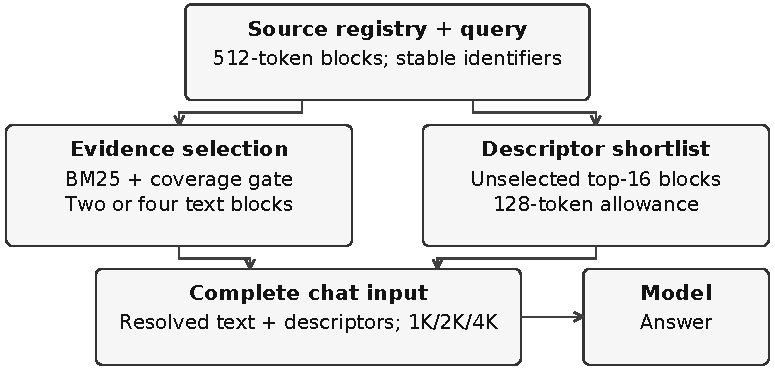
\includegraphics[width=\linewidth]{architecture.pdf}
\caption{SemPointer indexes source blocks, selects and resolves evidence, and adds bounded descriptors before the model answers.}\label{fig:architecture}
\end{figure}
\endgroup

BM25 ranks blocks, and the first two are protected. Let $T(q)$ contain the query terms and $T(S)$ the terms in the selected blocks. The coverage gate measures the fraction of positive inverse-document-frequency weight in the query represented in those blocks:
\begin{equation}\label{eq:coverage}
C_w(q,S)=\frac{\sum_{t\in T(q)\cap T(S)}\max(0,\operatorname{idf}(t))}{\sum_{t\in T(q)}\max(0,\operatorname{idf}(t))}.
\end{equation}
Equation~\eqref{eq:coverage} returns zero when its denominator is zero. The system requests four blocks when $C_w<0.70$, or when $C_w<0.90$ and the third BM25 score is at least 0.80 times the second. Block order breaks ties, and a 2,560-token resolved-text cap may reject candidates. Attention selection and semantic rescue are disabled.

The earlier full index grew with source length; bounding descriptors limits overhead. Selection determines expanded text, while descriptors expose a bounded view of unexpanded candidates.

The thresholds were selected on 36 fresh synthetic RULER development questions. The rule chose the lowest-token setting whose score was no more than two points below BM25-4. Three settings each scored 77.5, compared with 73.9 for BM25-4; the loose 0.70/0.90/0.80 setting used 1,815 mean input tokens versus 1,865 for the alternatives and was frozen.

A separate 30-question pilot selected a 128-token descriptor allowance over 256 at each budget by maximizing wins minus losses against budget-filling BM25. Ties favored coverage, fewer input tokens, and then the smaller allowance. For unexpanded blocks among the top 16 ranks, descriptors are admitted within that allowance. The full framed input, including instructions, labels, question, and chat template, must obey
\begin{equation}\label{eq:budget}
|\operatorname{ChatTemplate}(\operatorname{Frame}(q,X_S,D))|_{\rm tok}\leq L,
\end{equation}
where $X_S$ is the selected text, $D$ is the descriptor section, and $L$ is 1,024, 2,048, or 4,096 tokens. Equation~\eqref{eq:budget} counts the whole input, not just retrieved text. Blocks appear in source order; a final block can be clipped. Requests whose framing and question alone exceed the ceiling are skipped.
\section{Evaluation}
The bounded study uses pinned Qwen/Qwen3.5-4B with NF4 double quantization, BF16 compute, greedy non-thinking decoding, and batch size one on an 8-GB RTX 5060 Laptop GPU~\cite{dettmers2023qlora}. QA and non-CWE RULER outputs have a 128-token cap; common-word extraction (CWE) has a 512-token cap, and other tasks retain adapter-specific limits. Source guards exclude contexts exceeding two million characters or 262,144 model tokens.

The sample contains 100 questions each from RULER, LongBench, LoCoMo, LongMemEval, BABILong, LongBench v2, InfiniteBench, LooGLE, L-Eval, and SCROLLS~\cite{hsieh2024ruler,bai2024longbench,maharana2024locomo,wu2024longmemeval,kuratov2024babilong,bai2024longbenchv2,zhang2024infinitebench,li2024loogle,an2024leval,shaham2022scrolls}. Seed 20261118 balances available strata after earlier question IDs and pilot groups were excluded. The same 1,000 questions recur at all three budgets, with 859 exact contexts at 4K and only four LoCoMo conversations. Categories are restricted, sources recur (including all LoCoMo conversations), and eight families overlap earlier source groups. Pilot settings were frozen before the full run, but prior outcomes informed the design and tests are now exposed.

Four arms share the checkpoint and output caps: bounded pointers, adaptive selection without pointers, budget-filling BM25, and the original full index when it fits. Of 12,000 scheduled records, 9,941 were scored and 2,059 skipped; no inference errors were recorded. Comparisons use shared scored IDs. Task adapters use containment, exact or choice match, token-F1, ROUGE, and code metrics. LoCoMo and LongMemEval lexical adaptations and local SAMSum QA-F1 differ from official protocols. Because the metrics differ, we report per-question wins, ties, and losses (W/T/L), not pooled accuracy; a tie can be wrong in both arms. Generation time includes prefill and decoding but excludes ingestion and shared preparation. Cost savings are ratios of paired totals rather than averages of per-question percentage changes. These times do not measure end-to-end serving, throughput, or energy.

At 4K, a retrospective control compares saved pointer-on and pointer-off generations without new inference. Expanded text, IDs, question, references, source hash, output cap, and configuration match; removing the descriptor section reproduces the off prompt byte for byte. The smaller-budget comparisons can change expanded payload and do not provide this control. For overall net win balance we use 10,000 family-stratified, exact-context cluster bootstrap resamples. Exact-context clusters account for repeated questions but not every dependence among related sources. Task-level cluster sign-flip tests require five contexts; 53 of 123 groups qualify. Holm-adjusted results are exploratory, with a sensitivity analysis across all 123 groups assigning $p=1$ to untestable groups~\cite{holm1979}.
\section{Results}
Table~\ref{tab:budgets} shows the cost and coverage tradeoff. At 4K, bounded pointers use 54.2\% fewer input tokens and 42.7\% less generation time than budget-filling BM25, but lose on 229 questions and win on 123. Both systems share a ceiling, not an equal realized token count. At 1K the bounded index evaluates 972 questions versus six for the full index. It evaluates all 1,000 questions at 2K and 4K, versus 319 and 700 for the full index; coverage here means a request was evaluated, not answered correctly.

\begingroup
\renewcommand{\tablebodyfont}{\normalsize}
\renewcommand{\tablecaptionfont}{\small}
\begin{table}[!htbp]\centering
\caption{Bounded SemPointer versus budget-filling BM25 under three input ceilings. $n$ is the number of scored pairs; W/T/L counts quality wins, ties, and losses. Savings are ratios of paired totals.}\label{tab:budgets}
\begin{tabular*}{\linewidth}{@{\extracolsep{\fill}}rrrrr@{}}\toprule
\shortstack{Input\\ceiling} & $n$ & W/T/L & \shortstack{Tokens\\saved (\%)} & \shortstack{Generation\\saved (\%)} \\
\midrule
1,024 & 972 & 111/727/134 & 0.09 & 6.40 \\
2,048 & 1,000 & 132/686/182 & 17.90 & 13.65 \\
4,096 & 1,000 & 123/648/229 & 54.16 & 42.69 \\
\bottomrule\end{tabular*}\end{table}
\endgroup

Table~\ref{tab:families} reports all family-level quality outcomes. LongMemEval and LongBench v2 have positive win balances; most families favor BM25. Figure~\ref{fig:family-costs} shows cost reductions in every family, with input savings of 41.3--66.3\%. At 1K both prompts nearly saturate their ceiling; at 4K, budget-filling BM25 includes substantially more text. Cost savings do not establish quality equivalence.



\begingroup
\renewcommand{\tablebodyfont}{\normalsize}
\renewcommand{\tablecaptionfont}{\small}
\begin{table}[!htbp]\centering
\caption{Quality comparisons for every family at 4K, with 100 paired questions per row. Entries are wins/ties/losses. The descriptor comparison holds expanded evidence fixed and includes ten identical-input pairs.}\label{tab:families}
\begin{tabular*}{\linewidth}{@{\extracolsep{\fill}}lrr@{}}\toprule
Family & \shortstack{SemPointer versus\\budget-filling BM25} & \shortstack{Descriptors on\\versus off} \\
\midrule
RULER & 1/85/14 & 12/87/1 \\
LongBench & 11/58/31 & 10/69/21 \\
LoCoMo & 14/51/35 & 12/71/17 \\
LongMemEval & 16/73/11 & 10/80/10 \\
BABILong & 6/86/8 & 6/92/2 \\
LongBench v2 & 8/87/5 & 8/91/1 \\
InfiniteBench & 2/80/18 & 1/93/6 \\
LooGLE & 21/50/29 & 24/54/22 \\
L-Eval & 24/41/35 & 26/56/18 \\
SCROLLS & 20/37/43 & 25/47/28 \\
\bottomrule\end{tabular*}\end{table}
\endgroup

\FloatBarrier
\subsection{Descriptor Control}

Across 1,000 verified pairs, pointer-on records 134 wins, 740 ties, and 126 losses. Ten pairs have identical inputs and answers; the 990 active interventions give 134/730/126 W/T/L and a net win balance of $+0.81$ percentage points (clustered 95\% interval $[-2.47,3.96]$). Descriptors add 110.2 tokens, or 6.4\%, on average. Their overall utility is inconclusive. The intervention changes descriptor content, length, and token positions together, measuring the whole section rather than semantics alone. Its 1.6\% generation-time reduction is descriptive: pointer-on ran first in 742 pairs, leaving order sensitivity.

On 17 variable-tracking questions, scores rise from 37.65 to 74.12 (12 wins, five ties), a 36.47-point difference with exploratory clustered interval $[22.35,51.76]$. Descriptors expose gold names absent from expanded text in 14 cases, including 11 wins; gold is used only retrospectively. Every case has one chain and every assigned variable is a gold name, supporting entity recovery in this setting. Budget-filling BM25 scores 96.47. Raw sign-flip $p=0.000488$ becomes Holm $p=0.026$ across 53 eligible groups and $p=0.060$ across all 123 inspected groups. Their mean differences are positive/zero/negative in 25/76/22 groups; only variable tracking passes the narrower adjustment. Metrics and group sizes differ.
\begingroup
\renewcommand{\figurecaptionfont}{\small}
\begin{figure}[!htbp]
\centering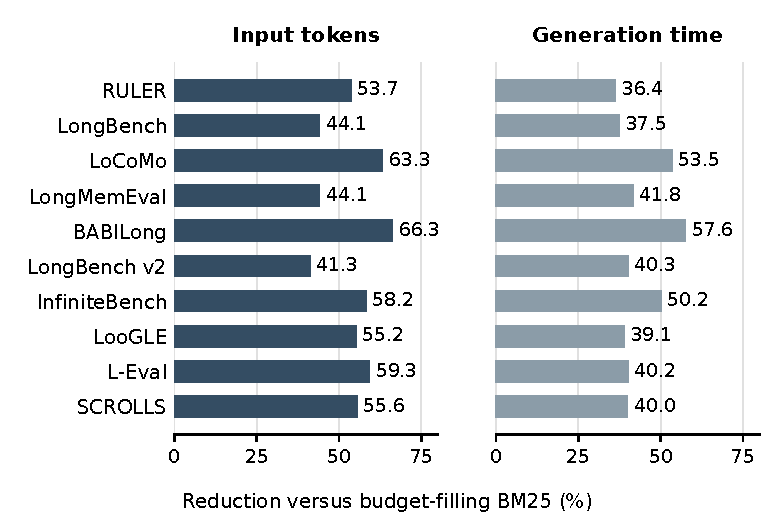
\includegraphics[width=\linewidth]{family_costs.pdf}
\caption{Input-token and generation-time savings by family versus budget-filling BM25 at 4K. Cost savings do not establish quality equivalence.}\label{fig:family-costs}
\end{figure}
\endgroup
\subsection{Separate Kaggle Evaluation}
A separate report snapshot uses the same pinned Qwen3.5-4B checkpoint with NF4/FP16 compute, batch size one, and two independent T4 workers. Eight subsets---BABILong, InfiniteBench, L-Eval, LoCoMo, LongBench, LongBench v2, LongMemEval, and LooGLE---each contribute 300 shared questions to the matched-budget comparison. RULER and SCROLLS remain partial and are excluded here. The figures reconcile within the combined report snapshot; the incomplete downloaded raw archive has not been independently audited.

Table~\ref{tab:kaggle} compares paired resource means. Against matched-budget BM25, SemPointer uses essentially the same mean input and has 8.9\% lower reported latency. Across 125 task groups, its mean native score is higher in 33, tied in 54, and lower in 38. These are directions of task-group means, not question-level W/T/L or a pooled accuracy measure. On 622 shared questions eligible for full context under a 16,384-token prompt guard, input and latency fall by 76.7\% and 61.3\%; across 68 task groups, mean scores are higher/tied/lower in 14/20/34. The 622-pair SemPointer means are reconstructed from task aggregates. Quality outcomes remain mixed.

\begingroup
\renewcommand{\tablebodyfont}{\normalsize}
\renewcommand{\tablecaptionfont}{\small}
\begin{table}[!htbp]\centering
\caption{Separate Kaggle snapshot: paired mean input tokens and reported latency. Each pair of rows uses the same questions; the two comparisons use different subsets.}\label{tab:kaggle}
\begin{tabular*}{\linewidth}{@{\extracolsep{\fill}}lrrr@{}}\toprule
System & Pairs & \shortstack{Mean input\\tokens} & \shortstack{Mean latency\\(s)} \\
\midrule
SemPointer & 2,400 & 4,071.4 & 5.504 \\
Matched-budget BM25 & 2,400 & 4,071.3 & 6.045 \\
\midrule
SemPointer & 622 & 1,875.1 & 4.865 \\
Full context & 622 & 8,038.8 & 12.564 \\
\bottomrule\end{tabular*}\end{table}
\endgroup

Table~\ref{tab:kaggle-quality} illustrates five comparisons selected after inspection. LoCoMo QA uses about 2,197 input tokens per arm. Paired example-bootstrap intervals are unadjusted for multiplicity and may understate uncertainty from shared sources. All include zero, establishing neither superiority nor equivalence. The source package retains the complete task inventory.

\begingroup
\renewcommand{\tablebodyfont}{\normalsize}
\renewcommand{\tablecaptionfont}{\small}
\begin{table}[!htbp]\centering
\caption{Illustrative Kaggle results on shared IDs (0--100 scale). $\Delta$: SemPointer minus matched BM25. Metrics: adapted QA F1 for the first three rows, first-line edit similarity without code execution for RepoBench-P, containment for KV. HotpotQA, Qasper, and RepoBench-P belong to LongBench. Differences use unrounded scores.}\label{tab:kaggle-quality}
\begin{tabular*}{\linewidth}{@{\extracolsep{\fill}}lrrrrr@{}}\toprule
Task & $n$ & \shortstack{Sem-\\Pointer} & \shortstack{Matched\\BM25} & $\Delta$ & \shortstack{Paired 95\%\\interval} \\
\midrule
LoCoMo QA & 300 & 24.73 & 24.69 & $+0.04$ & $[-2.52,+2.51]$ \\
HotpotQA & 27 & 73.28 & 68.13 & $+5.15$ & $[-5.65,+17.59]$ \\
Qasper & 8 & 50.15 & 39.48 & $+10.68$ & $[0.00,+31.78]$ \\
RepoBench-P & 26 & 24.69 & 20.94 & $+3.75$ & $[-1.54,+11.10]$ \\
InfiniteBench KV & 25 & 80.00 & 80.00 & $0.00$ & $[0.00,0.00]$ \\
\bottomrule\end{tabular*}\end{table}
\endgroup

Kaggle latency includes generation and measured selector cost, excluding shared ingestion and outer prompt preparation. It has no repeat-run interval and is not directly comparable to the local generation-only timings. This configuration is separate from the bounded 1K/2K/4K study. Fixed expanded payload has not been verified for its pointer-off arm, so it does not extend the local descriptor-control inference.
\section{Historical Comparisons and Protocol Checks}
The earlier three-collection study used Qwen2.5-3B NF4, thresholds 0.80/0.95/0.85, and output caps of 32 tokens for RULER and 64 for LongBench and LoCoMo. Its samples differ from those of the bounded study~\cite{qwen2025qwen25}. Table~\ref{tab:history} reports collection-specific scores and question-bootstrap intervals; these do not establish equivalence or account for source clustering. Relative to V1 on the same RULER questions, the score improved by 16.56 points, with an interval of $[11.00,22.56]$.

\begingroup
\renewcommand{\tablebodyfont}{\normalsize}
\renewcommand{\tablecaptionfont}{\small}
\begin{table}[!htbp]\centering
\caption{Original Qwen2.5-3B results. Scores use collection-specific metrics on a 0--100 scale. Differences are SemPointer minus BM25-4, with paired question-bootstrap intervals.}\label{tab:history}
\begin{tabular*}{\linewidth}{@{\extracolsep{\fill}}lrrrr@{}}\toprule
Collection & $n$ & \shortstack{Sem-\\Pointer} & BM25-4 & \shortstack{Paired difference\\(95\% CI)} \\
\midrule
RULER & 180 & 62.1 & 62.3 & $-0.22\ [-3.00,2.67]$ \\
LongBench & 600 & 10.4 & 10.6 & $-0.13\ [-1.04,0.79]$ \\
LoCoMo & 497 & 6.9 & 7.2 & $-0.37\ [-0.85,0.13]$ \\
\bottomrule\end{tabular*}\end{table}
\endgroup

Against BM25-4, the original study reduced input tokens by 8.9\%, 10.6\%, and 10.7\% on RULER, LongBench, and LoCoMo, respectively. Answer-call time fell by 15.7\%, 7.2\%, and 3.6\%. Those times include selection and prompt assembly as well as generation, unlike the newer generation-only measurements.

Against BM25-4, an intermediate Qwen3.5 full-index run on 936 shared questions records 137/624/175 W/T/L, uses 48.9\% more input tokens, and takes 21.4\% more generation time. Against its historical matched-token BM25 control on the same number of pairs, W/T/L is 140/611/185, the rounded input difference is $+0.00\%$, and generation time falls 6.00\%. Its mean 1,575-token index overhead motivated bounding; this is not a cross-model comparison.

A paired CWE audit covers 18 questions. At a 32-token cap, 17 SemPointer and all 18 BM25 outputs hit the cap; at 512 tokens neither does. Scores rise from 0 to 0.56 for SemPointer and 15.00 to 18.33 for BM25-4. This motivates the larger current CWE allowance, without establishing a general quality gain.
\section{Evidence Audit}
The audit aligns expanded text to frozen sources using tokenizer offsets. Table~\ref{tab:audit} partitions all 229 cases by annotation status. Only 43 have aligned fine annotations; in 18, bounded selection omits units fully retained by BM25. Annotated coverage does not establish contextual sufficiency, and these categories do not identify unique failure causes.

SCROLLS, LoCoMo, L-Eval, and LongBench account for 144 losses; 91 losses are summary tasks, including six SAMSum cases scored by local QA-F1. Spot checks show facts split across blocks: one bounded prompt includes block 6 but omits block 7, while BM25 includes both and returns the UUID. All nine variable-tracking losses have incomplete bounded chains; BM25 has complete chains in seven.

Among these losses, no bounded prompt hits the 4K input ceiling (mean 1,765 tokens), and only one answer hits its output cap. Boundary-preserving selection remains untested. Removing descriptors improves 94 selected losses and reaches BM25 in 47; this selected-subset result cannot establish an overall benefit.

Lexical scoring also affects interpretation. One LoCoMo answer includes the reference date 29 August 2023 but scores 0.286, below BM25's relative-date explanation at 0.375. These checks are not independent semantic rescoring or double-annotated causal labels; 229 metric losses are not 229 verified factual errors.

\begingroup
\renewcommand{\tablebodyfont}{\normalsize}
\renewcommand{\tablecaptionfont}{\small}
\begin{table}[!htbp]\centering
\caption{Evidence coverage among all 229 lower-scoring bounded cases at 4K. Coverage categories partition the cases but do not identify unique failure causes.}\label{tab:audit}
\begin{tabular*}{\linewidth}{@{\extracolsep{\fill}}p{.84\linewidth}r@{}}\toprule
Annotation status & Cases \\
\midrule
Fine evidence omitted by bounded selection, retained by BM25 & 18 \\
All annotated fine evidence present in bounded input & 9 \\
Fine evidence incomplete in both inputs & 16 \\
Coarse support-session labels only & 11 \\
No usable aligned fine annotation & 175 \\
\midrule
Total & 229 \\
\bottomrule\end{tabular*}\end{table}
\endgroup

\FloatBarrier
\section{Discussion and Limitations}
The local bounded study and the separate two-worker Kaggle run use one quantized checkpoint; they do not establish transfer across models. The local tests are exposed: earlier results informed the design, and fresh question IDs coexist with source reuse and limited category coverage. Exact-context clustering does not remove every dependency. Adapted lexical metrics restrict semantic interpretation and official benchmark comparability. The whole-section intervention changes prompt length and position as well as descriptor content, and the variable-tracking result is post hoc and sensitive to the multiplicity family. Kaggle adds a matched-budget comparator for its separate configuration; Adaptive-$k$ and a realized-token-matched comparator for the local bounded configuration remain untested. The timings do not establish serving throughput or energy savings, and the Kaggle snapshot awaits raw-database validation.

\section{Conclusion}
SemPointer provides a practical way to inspect and limit the evidence presented to a model. Bounded selection reduces cost across all sampled families. The separate matched-token Kaggle comparison also lowers reported latency, but neither result establishes uniform quality gains; the overall descriptor effect remains uncertain.

\section*{Code and Data Availability}
Earlier code: \url{https://github.com/VIKSIT-GARG/Sempointer}. Local records are retained under run \texttt{c73abaf595dc68e55696}; Kaggle aggregates under \texttt{8ef26bfd68509bae3b6b}. Newer raw records are not publicly archived. The source package includes Kaggle aggregates and provenance, including the pinned checkpoint revision; raw-archive validation remains pending.
\clearpage
\bibliography{references}
\end{document}
